\chapter{Reconhecimento Facial em Imagens} \label{chap:reco}

Neste capítulo é efetuada, em primeiro lugar, uma introdução ao problema de reconhecimento facial automático em imagens através de uma apresentação da sua evolução histórica. Posteriormente, é apresentada a definição do problema de reconhecimento facial automático, assim como dos sub-problemas que o compõem e dos desafios existentes para a sua resolução. Em terceiro lugar, são apresentadas as diversas áreas de aplicação do reconhecimento facial automático. De seguida, é efetuada uma revisão das estratégias utilizadas para a implementação deste tipo de sistemas, assim como das diversas soluções atualmente existentes. Por último, é efetuada uma revisão das avaliações efetuadas no âmbito dos programas FERET e FRVT e são apresentadas as conclusões retiradas destas avaliações.

\section{Evolução}
A capacidade de distinguir indivíduos através das suas características faciais é inata aos seres humanos, efetuada uma forma natural e quase sem esforço. A forma como efetuamos esse reconhecimento, é no entanto um problema complexo, que atrai a atenção de investigadores das mais diversas áreas, sendo da psicologia e na década de 50 \cite{BRUNERJEROMES.TAGIURI1954}, o mais antigo estudo efetuado sobre o tema. Associado a este problema, o reconhecimento facial automático, ou seja, o reconhecimento facial efetuado de uma forma automática com o auxílio de máquinas tais como computadores, tem de igual forma recebido muita atenção por tarte da comunidade científica, sendo que o primeiro sistema de reconhecimento facial automático de que há registo, foi desenvolvido da década de 70 por Takeo Kanade \cite{Kanade1973}. Ao longo dos anos, investigadores das mais diversas áreas, tais como  psicologia, reconhecimento de padrões, neurologia, visão por computador ou computação gráfica, efetuaram estudos em vários aspetos do reconhecimento facial efetuado por computadores e máquinas.

Ao nível do reconhecimento facial automático, após o trabalho de Kanade, e outros realizados por alguns dos seus pares na década de 70, verificou-se um abrandamento na investigação científica efetuada na área até meados dos anos 90, onde o trabalho realizado por Turk e Pentland \cite{Turk1991} trouxe um novo impulso ao desenvolvimento de sistemas e metodologias de reconhecimento facial automático. Neste estudo, Turk e Pentland apresentaram uma nova forma abordagem ao reconhecimento facial designada de \textit{Eingenfaces}. Um outro marco no desenvolvimento nas metodologias de reconhecimento facial, foi o surgimento do método \textit{Fisherfaces} \cite{Belhumeur1997, Zhao1998}, o qual apresenta uma maior insensibilidade em relação à variação da iluminação e expressões faciais presentes nas imagens.

Ao longo da década de 90 a investigação científica na área do reconhecimento facial automático intensificou-se, tendência que ainda se verifica atualmente, tal como pode ser verificado pelo surgimento de várias conferências, das quais são exemplo, desde as mais antigas
\textit{International Conference on Automatic Face and Gesture Recognition (AFGR)} (1995) e \textit{International Conference on Audio- and Video-Based Authentication (AVBPA)} (1997), até à recentemente realizada \textit{5th International Conference on Biometrics (ICBS)} (2012).

Paralelamente, o surgimento de programas como o Face Recognition Technology (FERET) (1993-1998), levado a cabo pelo \textit{National Institute of Standards and Technology (NIST)} dos E.U.A, com o objetivo de financiar a investigação na área e estabelecer padrões para a avaliação das diversas metodologias de reconhecimento facial criadas, assim como impulsionar a criação de uma base de dados de faces de grande dimensões para o teste dos sistemas criados, permitiu uma evolução significativa na área \cite{Phillips1998, Phillips2000}.

No final da década de 90, surgiram as primeiras aplicações comerciais de reconhecimento facial automático, tal como pode ser comprovado  pela participação de 5 soluções comerciais na primeira edição dos \textit{Facial Recognition Vendor Test (FRVT)}, no ano 2000 \cite{BlackburnDuaneM.;BoneMike;Phillips2001}. Nesta avaliação, as soluções eram testadas nas componentes de usabilidade e performance do reconhecimento efetuado, de modo fornecer uma avaliação objetiva e independente dos sistemas de reconhecimento facial presentes no mercado. Estas avaliações foram repetidas nos anos de 2002, 2006, 2010 e 2012.

\section{Definição do Problema} \label{sec:problema}
De uma forma geral, o problema de reconhecimento facial pode ser formulado da seguinte forma: dada uma imagem (prova), pretende-se identificar ou verificar a presença de uma ou mais pessoas na prova, comparando-a com uma base de dados de faces previamente guardada (galeria) \cite{Yang2002, Zhao2003}. Este problema, é ainda geralmente dividido em três subproblemas específicos: verificação de faces (ou autenticação), \textit{pair matching} e identificação de faces \cite{Li2011, Huang2007}:

\begin{description}
\item[Verificação] Uma prova é apresentada ao sistema, assim como a respetiva identidade da pessoa presente na imagem. Cabe ao sistema verificar se existe uma correspondência entre a pessoa representada na imagem e a identidade fornecida. Assim, é efetuada uma comparação 1:1, que responde à pergunta: "Esta pessoa é quem realmente afirma ser?".

\item[\textit{Pair Matching}] São apresentadas duas provas ao sistema, cada uma contendo uma face. O sistema deve decidir se as duas imagens correspondem, ou não, a representações da mesma pessoa. Tal como no sub-problema de verificação é efetuada uma comparação 1:1, a qual responde à pergunta: "Estas imagens pertencem à mesma pessoa?".

\item[Identificação] Uma prova é apresentada ao sistema, e pretende-se que este devolva a identidade da pessoa presente na imagem, assim como o nível de confiança associado à correspondência efetuada entre a imagem e a identidade devolvida. A identificação de faces pode ainda ser dividida em dois sub-problemas: 

No primeiro problema designado \textit{watch list} ou \textit{open-set identification}\cite{Chellappa2010}, não é garantido que o sistema conheça a pessoa a ser identificada, pelo que em primeiro lugar é necessário identificar se a pessoa existe na galeria e, caso exista, determinar a identidade da pessoa. Este sub-problema responde às perguntas: "Esta pessoa está presente na galeria? Se sim, de quem é esta face?". 

O segundo caso, é aquele que é geralmente avaliado em sistemas de reconhecimento facial, onde é garantido que a pessoa é conhecida pelo sistema, respondendo-se apenas à pergunta: "De quem é esta face?". Nesta situação, designada de \textit{closed-set identification}, podem ainda ser pedidas todas as correspondências efetuadas com um nível de confiança superior a um valor pré-definido. 

Em qualquer um dos subproblemas de identificação, é efetuada uma comparação 1:N.
\end{description}

Os sistemas de reconhecimento facial podem ainda ser divididos genericamente em dois grupos, tendo em conta a fonte de onde são extraídas as faces a analisar. O primeiro grupo baseia-se no uso de imagens estáticas, como por exemplo fotografias de personalidades ou mesmo em retratos de faces humanas criadas por ilustradores. O segundo, tem por base o uso de vídeos, dos quais são extraídas as faces a identificar ou verificar, sendo que neste caso essa identificação pode ainda ser efetuada em tempo real ou \textit{à posteriori}. No entanto, cada um destes meios representa problemas e desafios diferentes ao reconhecimento facial automático, pelo que devem ser estudados de forma individualizada, sendo que, no âmbito desta dissertação irá apenas ser abordado o sub-problema de reconhecimento facial efetuado em imagens estáticas.

\subsection{Sub-Problemas} \label{sec:sub-problemas}
O problema de reconhecimento facial em imagens é um problema complexo que obriga a que um conjunto de sub-tarefas sejam efetuadas com sucesso para uma identificação ou verificação eficaz da pessoa presente na imagem. Em primeiro lugar, é necessário determinar onde se encontra a face da pessoa a ser identificada, separando-a do resto da imagem. Posteriormente é necessário encontrar características que diferenciem essa face de outras. Finalmente, é ainda necessário efetuar a comparação da face, e respetivas características, com a galeria de imagens existente, fazendo assim o reconhecimento da pessoa representada. Este conjunto de sub-tarefas, são geralmente designados pelos seguintes passos fundamentais \cite{Zhao2003}:
\begin{description}
\item[Deteção:]
Determina a presença de uma face na imagem, e em caso positivo, efetua a sua segmentação do resto da imagem.

\item[Extração características faciais:]
Consiste na extração de características úteis para a diferenciação entre as diversas faces presentes no sistema. As características extraídas variam dependendo do método utilizado, podendo ir desde a distância entre olhos, à textura e cor da pele da pessoa a ser reconhecida, por exemplo. 

\item[Identificação ou Verificação]
Consiste na identificação ou verificação da identidade do sujeito presente na imagem tendo em conta as características extraídas e a informação presente no sistema.
\end{description}

Para além dos três passos mencionados anteriormente, existe ainda um quarto passo, efetuado após a deteção e antes da extração das características faciais, que merece destaque em alguns dos sistemas de reconhecimento facial existentes \cite{Li2011}:
\begin{description}
\item[Normalização]
Introduzida em alguns métodos de reconhecimento facial com o objetivo de melhorar os resultados do reconhecimento ao nível pose e iluminação das faces nas imagens. O seu objetivo consiste em normalizar a face geometricamente, ou seja na sua forma e enquadramento, e fotometricamente, ou seja ao nível da iluminação.
\end{description}
Na Figura \ref{fig:genericRF} é possível ver uma representação dos quatro passos fundamentais enunciados anteriormente que constituem um sistema de reconhecimento facial genérico. Em algumas soluções os passos de deteção e extração de características possuem possuem tarefas em comum, sendo realizados simultaneamente.

\begin{figure}[ht]
  \begin{center}
    \leavevmode
    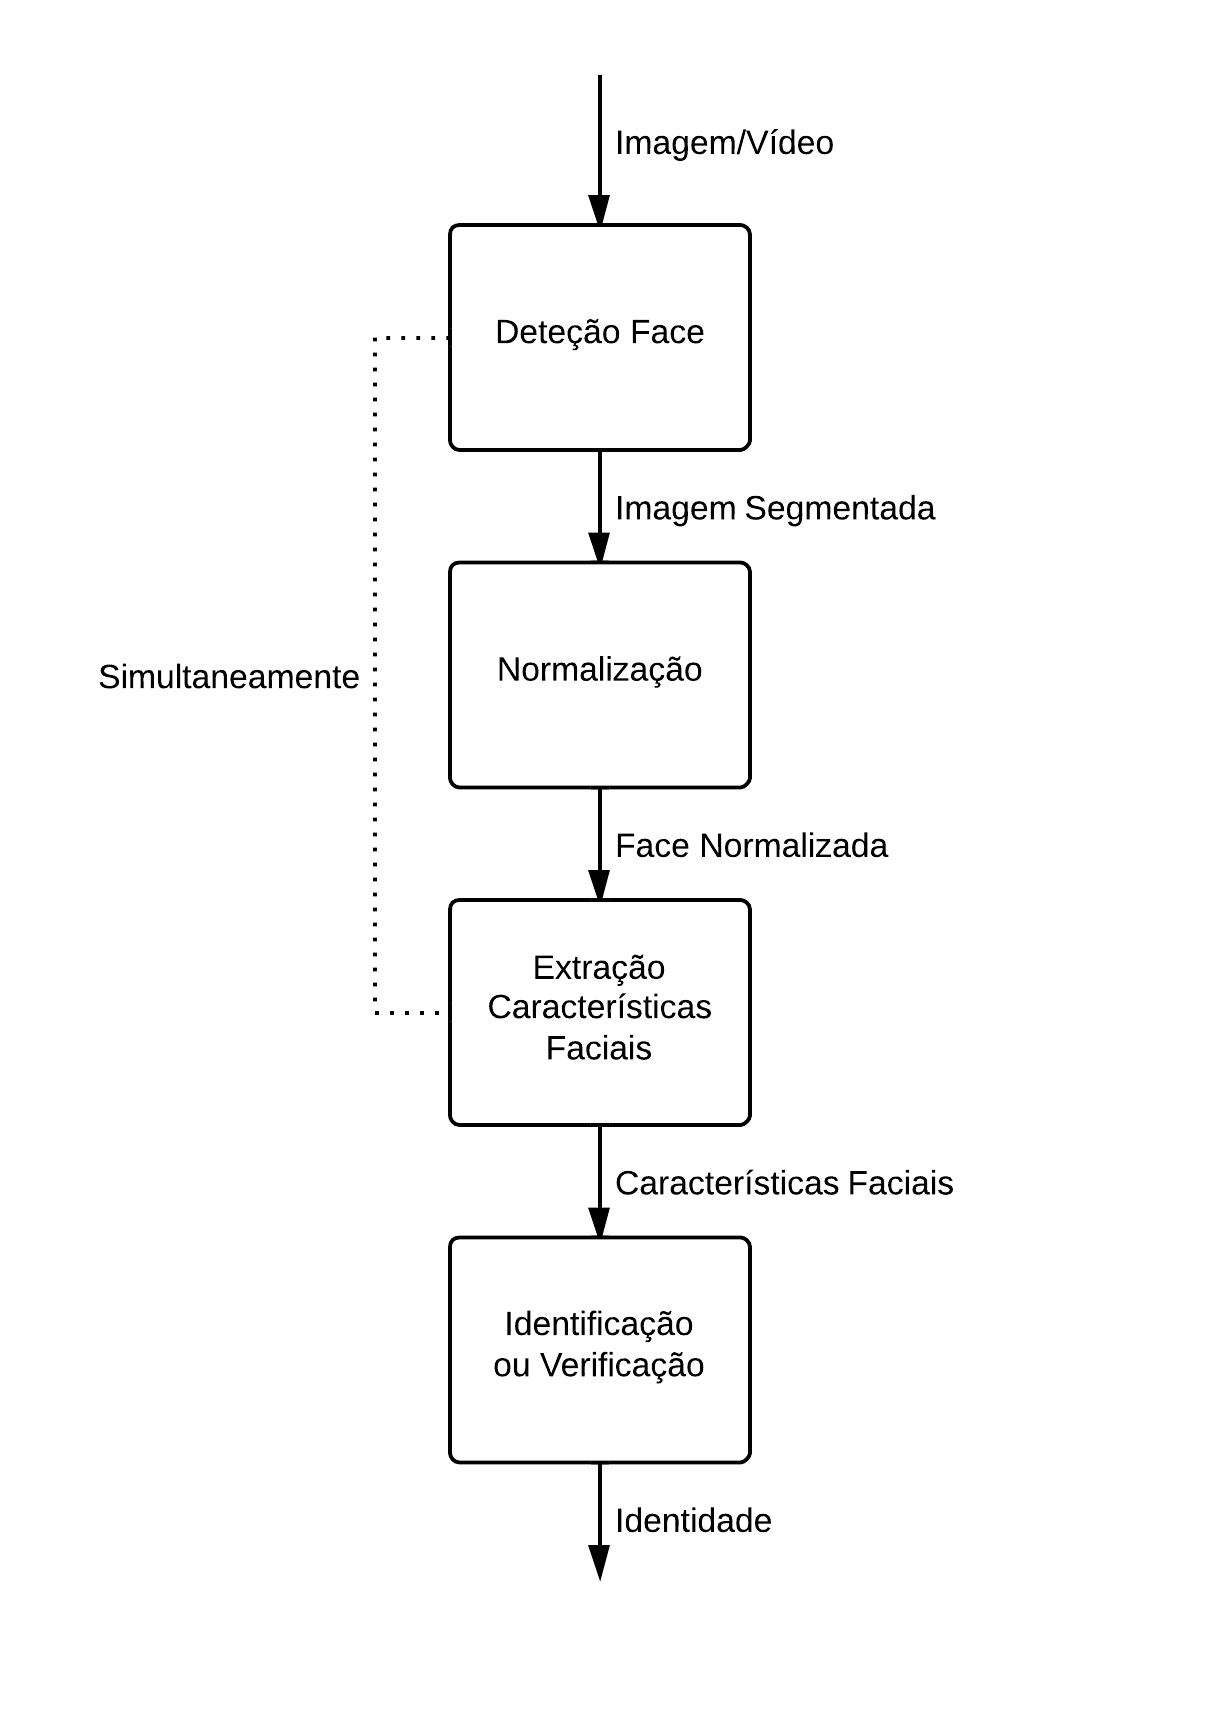
\includegraphics[width=0.5\textwidth]{SistemaGenericoRF}
    \caption{Sistema Genérico de Reconhecimento Facial}
    \label{fig:genericRF}
  \end{center}
\end{figure}

\subsection{Desafios} \label{desafios}
O reconhecimento facial automático em imagens é um problema complexo, sendo que existem um conjunto de desafios que se colocam na construção de um sistema de tipo. O primeiro passo em qualquer um desses sistemas, é a deteção de faces na imagem, a esse nível Yang \textit{et al.}, destacaram, no revisão ao estado da arte realizado em 2002,  os seguintes desafios \cite{Yang2002}:
\begin{itemize}
\item Pose e Orientação: A posição relativa da face à câmara pode sofrer uma grande variação dependendo do ambiente onde é capturada a imagem (variação no ângulo da face em relação à câmara vertical e horizontalmente, posição frontal, perfil). Ao variar a posição da face, alguns dos elementos que a permitem localizar e reconhecer podem ficar obstruídos. Avaliações efetuadas \cite{BlackburnDuaneM.;BoneMike;Phillips2001}, demonstram que este impacto é maior, quanto maior for o ângulo da pose em relação à posição frontal, sendo que uma variação até cerca de 25º não afeta significativamente os resultados do reconhecimento.
\item  Elementos Estruturais: a presença ou ausência de elementos estruturais, tais como barba ou óculos, assim como, a grande variação de forma e cor a que estes elementos podem apresentar afetam significativamente a forma como a face é percecionada pelo sistema.
\item Obstrução da face: as imagens captadas podem possuir objetos em frente à cara da pessoa a ser identificada, levando apenas a uma representação parcial da face na imagem.
\item Condições da imagem: aspetos como a resolução da imagem, o sensor utilizado para a captura e até mesmo eventuais defeitos associados à câmara utilizada podem potencialmente afetar o aspeto final da face na imagem.
\end{itemize}

Outro fator que afeta significativamente a perceção de uma face por um sistema de reconhecimento facial automático é a iluminação. Uma imagem pode ser capturada, com iluminação natural ou artificial. Para além disso, a iluminação pode estar sujeita a uma grande variação de tonalidades, intensidade e ângulo de incidência da luz.

Mesmo quando captadas pela mesma câmara, com as mesmas condições de iluminação e no mesmo local, podem existir variações significativas nas imagens captadas da face de uma pessoa devido às diferentes expressões faciais contidas nas imagens, fazendo com que este seja outro desafio a ultrapassar ao efetuar o reconhecimento facial automático.

O envelhecimento, ou eventuais alterações provocadas na face devido a fatores externos como por exemplo acidentes, exposição a condições extremas ou intervenção cirúrgica é outro dos fatores a ter em conta na identificação de uma pessoa.

Finalmente, existem ainda fatores como o elevado grau de semelhança entre pessoas com graus de parentesco próximos. Imagens capturadas de gémeos, ou até mesmo de pais e filhos, podem à primeira vista parecer imagens da mesma pessoa, tornando ainda mais difícil para um sistema automático efetuar a distinção dos indivíduos.

Assim sendo, para um reconhecimento fiável e eficaz é essencial que todas as etapas identificadas em \ref{sec:sub-problemas} sejam concluídas com sucesso. Sem uma correta deteção da presença de uma face na imagem, todos os passos subjacentes seriam impossíveis de ser realizados, por outro lado, o sucesso da extração das características faciais, encontram-se também dependente de uma normalização eficaz das imagens. No entanto, apesar desta dependência verificada entre as diversas etapas, cada uma delas representa problemas complexos, que devem a merecer a atenção e estudo de forma individual para que uma maior evolução das diversas técnicas envolvidas seja atingida \cite{Zhao2003}.


\section{Áreas de Aplicação}\label{sec:areasAplicacao}
O problema de reconhecimento facial automático tem merecido a atenção e estudo de inúmeros investigadores ao longo dos últimos 40 anos, motivados não só pelos desafios inerentes ao processo de reconhecimento facial, mas também pelas pela vasta gama aplicações onde a identificação de indivíduos é necessária \cite{Li2011}.

Adicionalmente, a evolução tecnológica da última década, permitiu a criação de sistemas computacionais mais poderosos, os quais tornaram possíveis desenvolvimentos na área que anteriormente seriam impensáveis gerando um ainda da maior interesse, tal como pode ser verificado pelo surgimento de uma vasta gama de aplicações comerciais e governamentais de reconhecimento facial, como é exemplo o sistema de fronteira automática dos aeroportos portugueses \cite{MinisteriodaAdministracaoInternaa}, assim como, pela recente aquisição de empresas da área do reconhecimento facial por parte de grandes empresas tecnológicas, nomeadamente Google e Facebook.

De seguida encontram-se descritas, em cinco categorias, algumas das áreas de aplicação do reconhecimento facial automático, respetivamente ilustradas com exemplos de aplicação real. Esta categorização foi baseada no estudo efetuado em \cite{Li2011}, o qual é para nosso conhecimento o mais recente estudo efetuado às diversas áreas de aplicação do reconhecimento facial, assim como em estudos anteriores efetuados por \cite{Zhao2003}. Esta secção pretende apenas apresentar de uma forma sumária algumas das possíveis áreas de aplicação, e respetivas soluções, às quais o reconhecimento facial poderá ser aplicado, não pretendendo ser um estudo exaustivo de todas as soluções existentes.

\subsection{Controlo de Acesso e Segurança de Informação} \label{sec:controloAcesso}
A necessidade de sistemas de fácil utilização que assegurem a segurança da nossa informação digital, assim como da privacidade dos utilizadores, sem que para isso seja necessário a memorização e utilização de um sem número de palavras-chave e códigos de segurança é premente. Neste campo, o reconhecimento facial destaca-se ao permitir a criação de sistemas de autenticação não invasivos que requerem um nível de cooperação baixo por parte dos participantes, em contraste com os sistemas tradicionais como o uso de palavras-chave, ou mesmo de sistemas mais complexos como a análise de impressões digitais, retina ou íris. Por outro lado, este tipo de sistemas, permite ainda determinar a presença factual do utilizador que se pretende identificar, e não apenas determinar o conhecimento de um código de acesso à informação.

Atualmente, o uso de reconhecimento facial para o controlo de acesso a informação encontra-se já a ser utilizado em diversas aplicações comercias como são exemplos os sistemas de autenticação disponíveis numa grande variedade de computadores portáteis. De uma forma geral, nestes sistemas,o utilizador apenas necessita de se aproximar do computador para que o reconhecimento facial e consequente autenticação sejam efetuados. Desta forma o utilizador não necessita de efetuar qualquer intervenção para aceder aos seus dados ou de memorizar qualquer palavra-chave.

O uso de reconhecimento facial para garantir uma maior segurança de informação, ou efetuar um mais eficaz controlo do seu acesso, é geralmente aplicado em soluções com um número de utilizadores limitado e nas quais as imagens capturadas apresentam baixa variabilidade nas condições de iluminação e pose dos utilizadores. Desta forma, o nível de precisão do reconhecimento atingido nesta área é normalmente elevado, fazendo com que o nível de satisfação dos seus utilizadores seja também elevado \cite{Li2011}.

\subsection{Cartões Inteligentes e Identificação de Faces} \label{CartoesInteligentes}
Os documentos pessoais inteligentes registam uma presença cada vez mais ativa na sociedade atual, como é caso do cartão do cidadão português (CC), que à data de 5 de Novembro de 2012 já tinha sido adotado por mais de 7 milhões de portugueses \cite{Administrativa}, ou mesmo do passaporte eletrónico português (PEP), o qual recebeceu igualmente uma ampla aceitação desde a sua criação em 2006 \cite{MinisteriodaAdministracaoInterna}.

Tradicionalmente, este tipo de documentos encontram-se dotados de capacidade de processamento e armazenamento próprios, podendo interagir com aplicações de terceiros como, por exemplo, sistemas de autenticação com recurso ao reconhecimento facial. O sistema designado de Reconhecimento Automático de Passageiros Identificados Documentalmente (RAPID)\cite{MinisteriodaAdministracaoInternaa}, desenvolvido pela empresa portuguesa Vision-Box \cite{Vision-Box} encontra-se desde 2007 em funcionamento nos vários aeroportos internacionais portugueses e tira partido das vantagens da associação da tecnologia de reconhecimento facial com documentos inteligentes. Em primeiro lugar, o sistema verifica se os dados armazenados no chip do passaporte são válidos, posteriormente, é efetuada uma comparação entre a fotografia armazenada no cartão e a imagem capturada do passageiro pelo dispositivo instalado na fronteira automática. Caso a identificação seja verificada, a porta que permite a passagem entre fronteiras é então automaticamente aberta. Todo o processo, encontra-se ainda a ser supervisionado por um operador numa cabine, o qual se encontra a supervisionar múltiplos dispositivos de identificação, sendo apenas necessária a sua intervenção quando não é efetuada uma identificação válida da pessoa.

O nível de precisão dos sistemas que tiram partido das sinergias entre cartões inteligentes e o reconhecimento facial apresenta uma correlação com o nível de atualização dos dados presentes nos documentos, sendo que  com um nível de atualização frequente é possível ser atingido um nível de satisfação elevado \cite{Li2011}, como se comprova pela bom funcionamento do sistema RAPID.
Contudo, esta é ainda uma área de investigação em aberto para que uma utilização destes sistemas de forma totalmente autónoma (sem que seja necessária a supervisão de um operador), em larga escala e, por exemplo, em ambientes não controlados seja possível.

\subsection{Entretenimento} \label{Entretenimento}
As tecnologias de reconhecimento facial apresentam uma forte potencialidade de aplicação nas área associadas ao entretenimento e à produção de conteúdos digitais, nomeadamente no que diz respeito à produção de jogos de computador e na interação humano computador.

As consolas modernas estão dotadas de capacidade de processamento notáveis, para além disso, juntamente com estas consolas é cada vez mais comum o surgimento de dispositivos como o \textit{Kinect} da Microsoft que permitem novas formas de interação e a criação de novos tipos de jogos. Uma das novidades introduzidas pelo \textit{Kinect} é a inclusão de diversos sensores e câmaras que permitem, entre outras coisas, efetuar um reconhecimento facial dos utilizadores. Desta forma, as equipas de desenvolvimento de jogos de computador, podem agora de uma forma mais fácil utilizar mecanismos de reconhecimento facial automático nos seus jogos de forma a criar jogos mais imersivos e personalizados. Este reconhecimento pode ainda ser aplicado ao nível da interação pessoa-computador  onde permite, a criação de sistemas com uma  uma maior facilidade de interação, uma vez que o próprio rosto poderá servir como um dispositivo de \textit{input} natural. 

À semelhança dos sistemas de controlo de acesso o reconhecimento facial automático na área do entretenimento é geralmente aplicado em soluções com um número de utilizadores limitado e onde o nível de precisão necessário não é muito alto fazendo assim com que a satisfação dos seus utilizadores seja, em geral, elevada \cite{Li2011}.

\subsection{Gestão de Conteúdos Multimédia e Bases de Dados} \label{GestaoMultimedia}
A sociedade atual caracteriza-se pelo constante fluxo de informação a que os seus indivíduos se encontram expostos. A título de exemplo e de acordo com dados divulgados pela Intel\cite{IntelCorporation}, a cada minuto, são visualizados no Youtube 1,3 milhões de vídeos e carregadas para os seus servidores 30 novas horas de vídeo. Já o Flicker, no mesmo período de tempo, regista a visualização de 20 milhões de fotos e o carregamento de 3000 novas imagens para a sua plataforma. Segundo os mesmos dados, atualmente o número de dispositivos com ligação à Internet é equivalente ao da população mundial e é esperado que em 2015 seja o dobro dessa população.

Este crescimento verificado quer na quantidade de conteúdos produzidos, quer na diversidade de dispositivos que acedem a esses conteúdos, torna assim extremamente importante uma gestão e organização eficazes dos mesmos. Os métodos tradicionais de pesquisa e organização de conteúdos multimédia baseiam-se em anotações textuais associadas a estes conteúdos. Com o uso de sistemas de reconhecimento facial é possível efetuar o reconhecimento das entidades presentes numa biblioteca multimédia mesmo que as suas fotografias não possuam qualquer anotação textual, uma vez que é feita uma análise da própria imagem e não apenas dos seus descritores, tornando-se assim um importante auxílio dos métodos tradicionais.

Atualmente existem no mercado diversas aplicações que permitem efetuar a organização de álbuns fotográficos  pessoais com recurso ao reconhecimento facial como por exemplo o Picasa da Google ou o iPhoto da Apple. Por outro lado, redes sociais como Google Plus e o Facebook, lançaram também recentemente serviços que permitem aos seus utilizadores a deteção e identificação automática de outros utilizadores presentes nas imagens carregadas para os seus servidores.

Apesar de a performance destes sistemas ter registado uma evolução notável nos últimos anos, a grande variabilidade associada às condições de captura de imagens e a grande quantidade de dados a ser processada faz com que exista ainda uma grande margem de evolução possível a este nível, sendo que a performance verificada ao nível do reconhecimento efetuado varia muito de acordo com a aplicação a analisar, assim como as características do conjunto de dados a organizar.

\subsection{Segurança e Aplicação da Lei} \label{sec:SegurancaAplicaçãoLei}
A preocupação com a segurança de instalações públicas e privadas, o controlo de emigração ilegal, a segurança de eventos com um grande impacto mediático ou mesmo o auxílio à investigação policial tornaram a segurança e aplicação da lei uma das áreas de aplicação que mais interesse despoletou por parte de sectores privados e governamentais desde o surgimento das primeiras tecnologias de reconhecimento facial.

Uma das aplicações mais comuns do reconhecimento facial em segurança é o reforço da vigilância da via pública. Desde 1998, diversas cidades implementaram sistemas de vigilância com recurso a reconhecimento facial, como são exemplos os sistemas instalados em \textit{Newham Borough of London}, \textit{Tampa (Florida)} e \textit{Virginia Beach (Virginia)} \cite{Li2011}.
Um outro exemplo, foi o sistema desenvolvido para os jogos olímpicos de 2008 em Pequim pela \textit{Chinese Academy Of Sciences} e que foi utilizado para validar as entradas nas cerimónias de abertura e encerramento dos jogos olímpicos \cite{ChineseAcademyOfSciences}.

A aplicação de sistemas de reconhecimento facial para a segurança e aplicação da lei tem atraído muita atenção por parte de sectores privados e governamentais, havendo o registo de alguns casos onde a sua aplicação se revelou um sucesso. Contudo, de uma forma geral estes sistemas debatem-se com um baixo nível de satisfação por parte dos seus utilizadores, isto porque, existe uma grande variabilidade nas condições de iluminação das imagens captadas, pose dos utilizadores, assim como, um número muito elevado de faces a analisar, resultando num número elevado de falsos positivos e consequentemente numa má performance dos sistemas \cite{Li2011}.

\section{Estratégias de Reconhecimento Facial}\label{sec:estratégias}
Após o trabalho inicial de Takeo Kanade em 1973 \cite{Kanade1973}, a área do reconhecimento facial automático passou um período de dormência até meados da década de 90, onde os trabalhos realizados recorrendo a métodos como Análise dos Componentes Principais (ACP) \textit{(Principal Component Analysis)}), Análise Linear Discriminante (ALD) \textit{(Linear Discriminant analysis)} e \textit{Elastic Graph Matching (EGM)}, revitalizaram a área \cite{Chellappa2010}. Ao nível da ACP, o método
 \textit{Eingenfaces} desenvolvido por Turk e Pentland em 1991 \cite{Turk1991}, foi um marco fundamental no rejuvenescimento do reconhecimento facial automático. Este método tira partido da redundância natural existente entre as representações faciais de diversos indivíduos, para através de uma análise dos componentes principais das faces, desenvolvida anteriormente por Kirby e Sirovich  \cite{Kirby1990}, efetuar uma representação de baixo nível das faces existentes. Posteriormente, o método \textit{Fisherfaces} \cite{Belhumeur1997, Etemad1997, Zhao1998}, que tira partido da aplicação de ALD após uma análise inicial dos componentes principais da imagem de forma a maximizar as variações entre indivíduos, apresentou também resultados positivos em experiências em bases de dados com um número elevado de faces a analisar. Finalmente, ao nível de EGM, foi percursor o trabalho realizado por Wiskott \textit{et al.} \cite{wiskott1997face}. No algoritmo EGM as faces são representadas como grafos, sendo cada nó posicionado em pontos fiduciais da face e a cada aresta associado um vetor de distância. A identificação de uma face consiste em determinar entre os grafos existentes aquele que maximiza a função de similaridade entre grafos.
 
Desde então, diversos investigadores estenderam estes três tipos de algoritmos. Em 2003, Zhao \textit{et al.} \cite{Zhao2003} efetuaram um estudo aprofundado das técnicas desenvolvidas até então classificando-as em três categorias. Métodos holísticos, caso estes usem toda a região da face como fonte de comparação no reconhecimento, métodos baseados nas caraterísticas faciais, caso estes usem as características extraídas como informação essencial para a classificação da face e ainda como híbridos, caso seja utilizada uma mistura de ambos os métodos. Os resultados desta classificação podem ser visualizados na Tabela \ref{tabelaZhao}.

\begin{center}
\begin{table}
	\caption{Categorização dos Métodos de Reconhecimento Facial em Imagens por Zhao \textit{et al.} \cite{Zhao2003}}
	% title of Table
	\centering
	% used for centering table
	\begin{tabular}{l p{8cm}}
	% centered columns (4 columns)
	\hline\hline
        Método                     & Trabalho Representativo\\
	% inserts table
	%heading
	\hline
		% inserts single horizontal line
Holistic methods	 \\	
$\quad$ \textit{Principal Component analysis (PCA)} \\
$\qquad$  Eigenfaces                 & Direct application of PCA [Craw and Cameron 1996; Kirby and Sirovich 1990; Turk and Pentland 1991] \\
$\qquad$        Probabilistic eigenfaces   & Two-class problem with prob. measure [Moghaddam and Pentland 1997] \\
$\qquad$        Fisherfaces/subspace LDA   & FLD on eigenspace [Belhumeur et al. 1997; Swets andWeng 1996b; Zhao et al. 1998] \\ 
$\qquad$        SVM                        & Two-class problem based on SVM [Phillips 1998] \\ 
$\qquad$        Evolution pursuit          & Enhanced GA learning [Liu andWechsler 2000a] \\ 
$\qquad$        Feature lines              & Point-to-line distance based [Li and Lu 1999] \\ 
$\qquad$        ICA                        & ICA-based feature analysis [Bartlett et al. 1998] \\ 
$\quad$ \textit{Other Representations} \\
$\qquad$        LDA/FLD                    & LDA/FLD on raw image [Etemad and Chellappa 1997] \\ 
$\qquad$        PDBNN                      & Probabilistic decision based NN [Lin et al. 1997] \\

Feature-based methods \\
$\qquad$        Pure geometry methods      & Earlier methods [Kanade 1973; Kelly 1970]; recent methods [Cox et al. 1996; Manjunath et al. 1992] \\ 
$\qquad$        Dynamic link architecture  & Graph matching methods [Okada et al. 1998;Wiskott et al. 1997] \\ 
$\qquad$        Hidden Markov model        & HMM methods [Nefian and Hayes 1998; Samaria 1994; Samaria and Young 1994] \\

Hybrid methods \\
$\qquad$        Convolution Neural Network & SOM learning based CNN methods [Lawrence et al. 1997] \\ 
$\qquad$        Modular eigenfaces         & Eigenfaces and eigenmodules [Pentland et al. 1994] \\ 
$\qquad$        Hybrid LFA                 & Local feature method [Penev and Atick 1996] \\ 
$\qquad$        Shape-normalized           & Flexible appearance models [Lanitis et al. 1995] \\ 
$\qquad$        Component-based            & Face region and components [Huang et al. 2003] \\
        \hline
    \end{tabular}
	\label{tabelaZhao}
\end{table}
\end{center}
 
 Tal como referido na Secção \ref{desafios} deste relatório, o reconhecimento facial é uma tarefa complexa, composta por um conjunto de sub-problemas que enfrentam uma série de desafios para a sua conclusão. O primeiro desafio em qualquer sistema de reconhecimento facial é a deteção da face na imagem, a esse nível o trabalho realizado por Paul Viola e Michael Jones \cite{Viola2004} é considerado como um dos mais robustos métodos disponíveis na atualidade. Outras áreas onde a investigação atual se encontra focada têm a ver com a criação de métodos de reconhecimento facial robustos em relação à iluminação das imagens, assim como a pose dos indivíduos representados. \cite{Chellappa2010}.
 
 Ao nível da pose, o uso de  \textit{3D morphable face models} \cite{Blanz2003} tem revelado resultados positivos em posições não frontais. Estes algoritmos simulam o processo de formação de uma face em 3D, estimando a sua representação tridimensional com recurso a técnicas de computação gráfica, a partir de imagens 2D fornecidas ao sistema. Esta estimativa é efetuada através do encaixe de um modelo 3D de faces na própria imagem fornecida, modelo esse apreendido através da digitalização 3D de um conjunto de rostos e respetiva textura. No entanto, em grande parte dos modelos desenvolvidos a seleção manual de um pequeno número de características faciais é requerida e o poder de computação necessário para a criação dos modelos é elevado. Extensões destes modelos foram também propostas para criar sistemas mais robustos em relação à variação na iluminação \cite{Chellappa2010}.  
 
 Outras abordagens que têm em vista a criação de sistemas de reconhecimento facial robustos em relação à iluminação centram os seus esforços na estimação do albedo para a normalização das imagens. O albedo representa a relação entre a quantidade de luz refletida por um ponto e quantidade de luz incidente, métodos recentes centram-se no desenvolvimento de filtros estocásticos não estacionários para a estimação de mapas de albedo das amostras faciais \cite{Biswas2009}. Estes mapas podem ainda ser combinados com os modelos 3D faciais desenvolvidos para uma representação facial mais completa. Apesar de os resultados obtidos por estes métodos serem promissores quando comparados com os métodos tradicionais como o \textit{Eigenfaces}, estes métodos ainda carecem de maior validação, uma vez que as suas avaliações foram feitas utilizando conjuntos de dados controlados e de reduzida dimensão \cite{Chellappa2010}.
 
O investimento realizado na investigação de metodologias de reconhecimento facial automático tem permitido progressos notáveis na área. Do mesmo modo, a investigação em áreas relacionadas como a deteção de faces nas imagens, o envelhecimento facial ou o reconhecimento de expressões faciais em imagens tem permitido evoluir ainda mais os resultados obtidos. Devido à complexidade envolvida no processo de reconhecimento facial automático a evolução na área encontra-se assim intrinsecamente ligada à evolução verificada nas múltiplas áreas envolvidas, sendo que a investigação independente de cada uma dessas áreas é crítica para uma resolução eficaz da grande variabilidade de desafios que o reconhecimento facial automático se propõe ultrapassar.

\subsection{Soluções Existentes}\label{sec:soluções}
A investigação desenvolvida nos vários centros de investigação na década de 90, levou à passagem das soluções de reconhecimento facial automático de meros protótipos laboratoriais, para soluções comerciais de elevado valor acrescentado, dessas soluções resultaram três categorias comerciais de produtos na área do reconhecimento facial:
\begin{itemize}
\item Soluções Completas. Estas soluções caracterizam-se por oferecer toda a infraestrutura necessária para efetuar o reconhecimento facial, quer a nível de software, quer a nível de hardware.
\item Software. Soluções tradicionais de sistemas de reconhecimento facial, que consistem em software que permite efetuar o reconhecimento facial independentemente do hardware utilizado para a captura de informação.  Dentro destas soluções existe uma grande variedade nos produtos oferecidos, desde soluções baseadas na captura de imagens 2D estáticas, imagens 3D e vídeo. Para além disso, as soluções oferecidas encontram disponíveis para serem utilizadas em diversas plataformas, como por exemplo dispositivos móveis ou através da Internet.
\item \textit{Software Development Kit (SDK)} de reconhecimento facial. Permitem aos clientes, a criação de novas soluções de reconhecimento facial a partir de módulos independentes ou APIs desenvolvidas por terceiros.
\end{itemize}

Para além do reconhecimento facial automático, as soluções disponíveis possuem muitas vezes também associados outros métodos de biometria, como por exemplo reconhecimento de íris ou impressões digitais, assim como métodos mais tradicionais de autenticação como o uso de cartões de identificação ou passwords, de modo a aumentar a robustez e segurança dos sistemas.
Na Tabela \ref{tab:mbe2010}, encontram-se listadas as soluções participantes na última avaliação, para a qual existem dados disponíveis, realizada a sistemas de reconhecimento facial automático em imagens.

\begin{center}
\begin{table}
	\caption{Participantes na avaliação MBE 2010 \cite{Grother2010}.}
	% title of Table
	\centering
	% used for centering table
	\begin{tabular}{l p{8cm}}
		\hline\hline
		Empresa/Organização             & Website                                  \\ \hline
		Cognitec                        & \url{http://www.cognitec-systems.de}           \\ 
		Dalian University of Technology & \url{http://www.dlut.edu.cn}                   \\ 
		L1 Identity Solutions           & \url{http://www.l1id.com} \footnote{Integrada no grupo Morphotrust USA - http://www.morphotrust.com}                      \\ 
		NEC                             & \url{http://www.nec.com/en/global/solutions/security/technologies/face_recognition.html}                       \\ 
		Neurotechnology                 & \url{http://www.neurotechnology.com}           \\ 
		Pittsburg Pattern Recognition   & \url{http://www.pittpatt.com} \footnote{Adquirida pela Google Inc.}                  \\ 
		Sagem                           & \url{http://www.sagem.com} \footnote{Integrada no grupo Morphotrust USA - http://www.morphotrust.com}                     \\ 
		Surrey University               & \url{http://www.surrey.ac.uk}                  \\ 
		Toshiba                         & \url{http://www.toshiba.com}                   \\ 
		Tsinghua University             & \url{http://www.tsinghua.edu.cn}               \\
		\hline
    \end{tabular}
	\label{tab:mbe2010}
\end{table}
\end{center}

Para além das soluções comerciais de reconhecimento facial ao longo dos últimos anos surgiram também algumas soluções gratuitas de reconhecimento facial. Deste tipo de soluções são exemplo o software Picasa da Google, ou software iPhoto da Apple que permitem aos seus utilizadores a organização de álbuns multimédia com recurso ao reconhecimento facial. Por outro lado, redes sociais como Google Plus e o Facebook, lançaram também recentemente serviços que permitem a deteção e identificação automática de utilizadores presentes nas imagens carregadas para os seus servidores. Finalmente ao nível das plataformas de desenvolvimento, existem também alguns sistemas de código aberto, sendo que a este nível se destaca a biblioteca \textit{OpenCV}, pelo seu grau de maturidade, grande número de utilizadores e dimensão da comunidade de suporte.
\footnotetext[1]{Integrada no grupo Morphotrust USA - http://www.morphotrust.com}

\footnotetext[2]{Adquirida pela Google Inc.}

\footnotetext[3]{Integrada no grupo Morphotrust USA - http://www.morphotrust.com}

\section{Análises de Desempenho Efetuadas}\label{sec:performance}
O desempenho de um sistema de reconhecimento facial depende de uma grande variedade de fatores como a iluminação, posição da face na imagem, expressão facial e presença ou ausência de adereços (ex:óculos) na face. Por outro lado, as condições de utilização do próprio sistema, tais como o número de utilizadores diferentes e a frequência de utilização, são também fatores a ter em conta ao avaliar a performance de um sistema. Uma avaliação apropriada dos sistemas de reconhecimento facial encontra-se então dependente da existência de uma base de dados de grandes dimensões e consequentemente um conjunto de casos de teste vasto, assim como, da existência de métodos apropriados para essa avaliação.

A criação do programa FERET em 1993, pelo NIST, permitiu assim colmatar uma lacuna existente na avaliação dos sistemas de reconhecimento facial existentes com a criação de uma base de dados de faces de grande dimensões assim como de um protocolo de avaliação dos respetivos sistemas de reconhecimento facial. Com base no protocolo desenvolvido foram levadas a cabo avaliações aos nos anos de 1994 e 1995. Um novo protocolo foi criado para a avaliação realizada em 1996. Posteriormente, o mesmo instituto realizou novas avaliações baseadas no protocolo FERET96 na edição de 2000 dos FRVT, a partir de 2002, um outro protocolo foi criado (protocolo FRVT 2002), com base no protocolo FERET96, mas com a particularidade de permitir a avaliação de sistemas de biometria em geral e não apenas sistemas de reconhecimento facial. Com base no novo protocolo criado foram então realizadas avaliações nos anos de 2002, 2006 e 2010. A decorrer encontram-se ainda as avaliações FRVT 2012, para as quais ainda não existem à data resultados divulgados.

As avaliações levadas a cabo durante os programas FERET e FRVT constituem desta forma uma boa base para a análise da evolução dos sistemas de reconhecimento facial automático ao longo dos últimos 20 anos, tal como pode ser visto na Figura \ref{fig:evolucaoAvaliacoes}. De seguida encontram-se descritas os principais objetivos e conclusões retiradas dos programas FERET e FRVT:

\subsection{FERET}
Para além dos objetivos anteriormente citados de criação de uma base de dados de grandes dimensões e de criação de um protocolo que permitisse uma avaliação concreta e de base científica dos algoritmos existentes, o programa FERET tinha ainda como propósitos avaliar o estado da arte e identificar futuras áreas de desenvolvimento do reconhecimento facial \cite{Phillips2000}. Tendo em conta estes objetivos, foi então avaliada a performance dos diferentes algoritmos em diferentes cenários, categorias de imagens e diferentes versões dos próprios algoritmos. A performance foi computada para situações de identificação e verificação de faces, estando os principais resultados da última avaliação, efetuada em 1996, descritos em Phillips \textit{et al.} \cite{Phillips2000}.

A primeira avaliação do programa FERET, em 1994, consistia num três de conjuntos de testes, cada um com uma galeria e conjunto de provas diferentes. O primeiro conjunto, consistia numa prova de reconhecimento de faces de uma galeria de 316 faces. O segundo, tinha com objetivo determinar a capacidade dos algoritmos de rejeitar faces não presentes na galeria, designadas de falso-alarme. O terceiro, tinha como objetivo analisar os efeitos da pose na performance dos algoritmos \cite{Phillips2000}.

Em 1995, teve lugar a segunda avaliação, com o objetivo de  avaliar os mesmo algoritmos em galerias de maior dimensão. A performance foi medida num único teste, com uma galeria de 817 indivíduos conhecidos, tendo sido dado um maior ênfase na avaliação de provas duplicadas. Um duplicado é uma imagem cuja imagem correspondente da galeria foi geralmente capturada em dias diferentes  \cite{Phillips2000}.

Na última edição, em 1996, e já com um protocolo atualizado, foram testados 12 algoritmos de reconhecimento facial, e estudada a sua performance em quatro situações diferentes, usando para isso uma galeria com um total de 1196 indivíduos. Na primeira situação, a galeria e as imagens de prova foram tiradas no mesmo dia e sobre as mesmas condições de iluminação. No segundo conjunto de provas, a galeria e as imagens de prova foram tiradas em dias diferentes. Para o terceiro teste, a galeria e as respetivas provas foram capturadas com pelo menos um ano de diferença. Finalmente, no quarto e último conjunto de testes, a galeria e as imagens de prova forma tiradas no mesmo dia, mas com diferentes condições de iluminação.

Várias conclusões foram retiradas das avaliações efetuadas. A primeira conclusão foi que, de facto, se verificava uma evolução nas técnicas de reconhecimento facial, uma vez que os resultados foram progressivamente melhores, mesmo quando comparadas versões diferentes do mesmo algoritmo. Essa conclusão é suportada pela análise dos resultados do caso geral de identificação, testado em todas as edições, onde as imagens da galeria e da prova foram capturadas no mesmo dia e com a mesma iluminação. Nesse teste em 1994, apenas 78\% indivíduos foram identificados com sucesso numa galeria de 317 indivíduos, ao passo que em 1995 foram identificados já 93 \% dos indivíduos numa galeria de 831 e nos testes da última edição (1996), 95\% dos indivíduos foi identificado numa galeria de 1196 indivíduos. De igual forma, foi também verificada evolução na deteção de duplicados, mantendo-se no entanto as percentagens de identificação de duplicados mais reduzidas quando comparadas com o caso geral de identificação devido à maior complexidade do problema.

Outra conclusão retirada foi que a performance se encontra dependente da galeria e conjunto de imagens de prova utilizadas, uma vez que foi verificado que mudando a galeria, mas mantendo o mesmo tipo de teste a ser efetuado a percentagem de indivíduos identificados varia significativamente. Para a galeria e conjunto de prova capturadas no mesmo dia a percentagem varia entre os 80\% e os 94\%, enquanto que para galeria e conjunto de prova, capturadas em dias diferentes essa percentagem varia entre os 24\% e os 69\% porcento. Para além disso, não se existiu qualquer algoritmo que se revelasse superior em todas as quatro situações de teste realizadas em 1996, variando as performances, conforme a situação de teste.

Finalmente, conforme a tarefa a efetuar, identificação ou verificação de faces, ficou também demonstrado que não havia uma técnica que se superiorizasse em ambas as situações, comprovando que o reconhecimento facial é uma tarefa complexa que necessita de um estudo e investigação concretos tendo em conta a área de aplicação em vista.

\subsection{FRVT}
Durante a década de 90 registou-se um progresso assinalável nas diversas técnicas de reconhecimento facial, tendo para isso sido muito importante o papel desempenhado por iniciativas como o FERET. No final da década de 90, assistiu-se então a uma passagem dos sistemas de reconhecimento facial existentes de meros protótipos universitários, para aplicações comerciais de reconhecimento facial automático, tal como pode ser comprovado  pela participação de 5 soluções comerciais na primeira edição dos \textit{Facial Recognition Vendor Test}, no ano 2000. Esta avaliação, tinham como objetivo maioritário efetuar uma avaliação técnica das capacidades dos sistemas comerciais de reconhecimento facial disponíveis, de forma a compreender os pontos fortes e fracos de cada sistema, obtendo também uma análise do estado da arte do reconhecimento facial à data \cite{BlackburnDuaneM.;BoneMike;Phillips2001}. Estas avaliações foram ainda repetidas em 2002, 2006, 2010 e ainda em 2012.

A primeira edição dos FRVT, em 2000, utilizou o mesmo protocolo de avaliação da avaliação última avaliação FERET em 1996, no entanto, os testes efetuados eram significativamente mais exigentes do que a avaliação anterior, sendo utilizada também uma muito maior variedade de imagens. Os resultados da avaliação efetuada foram ser reportados para as seguintes oito categorias: compressão, distância, expressão,  media, iluminação, pose, resolução e variação temporal. Ao nível das conclusões retiradas, podem ser destacados os seguintes tópicos \cite{BlackburnDuaneM.;BoneMike;Phillips2001, Chellappa2010, Li2011}:
\begin{itemize}
\item Compressão de imagens, utilizado JPEG, até 40:1 não reduziu a taxa de reconhecimento;
\item Pose não afeta o reconhecimento de forma significativa até $\pm$ 25º, mas afeta significativamente quando são atingidos os $\pm$ 40º;
\item De forma equivalente ao registado no programa FERET, o uso de diferentes iluminações interiores não afeta significativamente os resultados obtidos, no entanto esses resultados são afetados caso haja uma mudança entre zonas interiores e exteriores;
\item Registou-se uma melhoria significativa dos resultados obtidos em imagens tiradas com mais de 18 meses de distância, quando comparado com os resultados obtidos no FERET. (Aumento de 5\% a 12\% de faces identificadas conforme o conjunto de dados avaliado).
\end{itemize}

A segunda edição dos FRVT teve lugar em 2002, contou com a participação de soluções de reconhecimento facial de 10 empresas distintas. Esta edição consistiu em duas provas fundamentais, os \textit{High Computational Intesity test (HCInt)} e os \textit{Medium Computational Intensity test (MCInt)}. Os HCInt tinham como objetivo medir a performance dos sistemas existentes em 121 589 imagens frontais de 37 435 pessoas, representando um desafio computacional de elevado grau de exigência, como comprovado pelas 242 horas de computação necessárias para efetuar os testes. Os \textit{Medium Computational Intensity test (MCInt)}, assemelhavam-se às medições efectuadas em avaliações anteriores, como o FERET e o FRVT 2000, tendo como objetivo medir a performance dos sistemas em imagens de diferentes categorias, nomeadamente não frontais, capturas no interior e exterior, entre outros. As conclusões retiradas desta avaliação foram as seguintes \cite{Chellappa2010, Li2011}:
\begin{itemize}
\item Melhores sistemas são insensíveis a variações de luz interior;
\item Reconhecimento facial em imagens exteriores é ainda um desafio por resolver;
\item Utilização de \textit{3D morphable models} melhora a performance em situações não frontais;
\item Características como sexo e idade podem afetar significativamente a performance, sendo que se registou maior facilidade em distinguir homens e pessoas com idade superior.
\item O tempo de captura entre provas afeta significativamente a performance, registando-se uma diminuição linear da performance com o aumento do tempo.
\end{itemize}

As últimas edições dos FRVT para as quais foram divulgados resultados foram as edições de 2006 \cite{Phillips2007} e a de 2010. Na edição de 2010 a competição não assumiu o nome de FRVT 2010, mas sim de \textit{Multiple Biometric Evaluation (MBE)} 2010-\textit{still image track}, uma vez que além de avaliados sistemas de reconhecimento facial automático foram também avaliados sistemas de biometria com base na análise da íris. \cite{Grother2010}. Foi também realizada uma edição dos FRTV em 2012, mas a avaliação dos sistemas ainda se encontra a decorrer, não havendo por isso resultados divulgados.

\begin{figure}[t]
  \begin{center}
    \leavevmode
    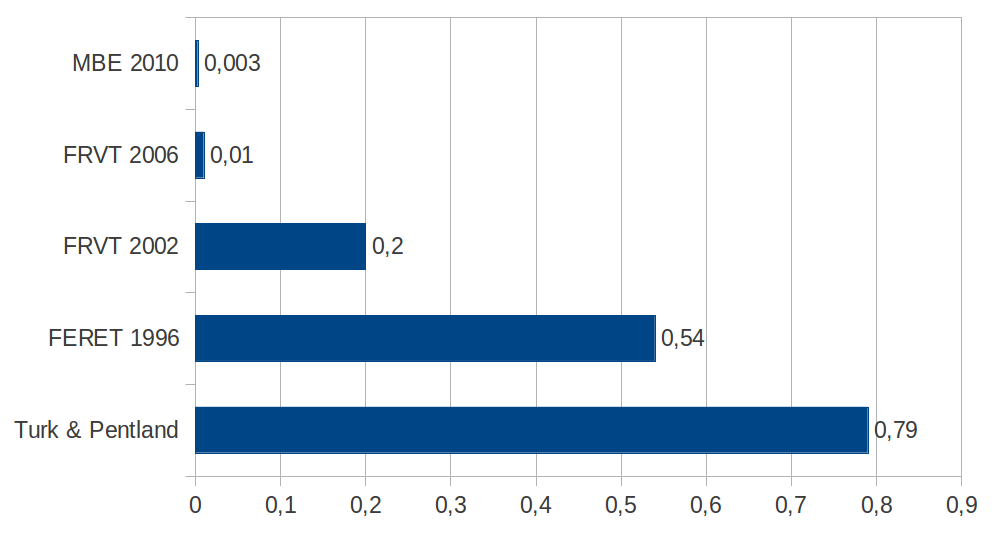
\includegraphics[width=0.9\textwidth]{EvolucaoAvaliacoes}
    \caption{A redução da taxa de erro para os algoritmos estados da arte tal como documentado nas avaliações FERET, FRVT 2002, FRVT 2006 e MBE 2010 \cite{Phillips2007, Grother2010}}	
    \label{fig:evolucaoAvaliacoes}
  \end{center}
\end{figure}

Em 2006, foi analisada a performance de sistemas de reconhecimento facial, de 22 organizações e de 10 países diferentes, baseados em representações 3D e em imagens estáticas de faces. As avaliações consistiam em três testes distintos: comparação de imagens capturadas com luz interior; comparação de digitalizações de faces 3D com base na forma e textura; comparação de imagens capturadas em estúdio com imagens capturadas em corredores e átrios. Em 2010, para além do conjunto de dados analisados em 2006 e 2002, de modo a averiguar a evolução comparativa dos algoritmos, foi também analisado um segundo conjunto de imagens recolhidas por várias agências de segurança e compiladas pelo \textit{Federal Bureau of Investigation (FBI)}. Este segundo conjunto de dados possuía mais de 1 milhão de faces fazendo da avaliação de 2010 a avaliação em maior escala feita aos sistemas de reconhecimento facial à data. Das provas de 2006 e 2010, as principais conclusões obtidas foram as seguintes \cite{Phillips2007, Grother2010, Chellappa2010, Li2011}:
\begin{itemize}
\item Desde 1993 foram atingidas melhorias de 2 ordens de magnitude;
\item Os resultados de 2010 e 2002 mostram uma melhoria de 1 ordem de magnitude nos sistemas de reconhecimento facial (Para um \textit{false accept rate (FAR)} de 0.001, foi registado em 2002 um \textit{false reject rate (FRR)} de 0.2, enquanto que em 2010 FRR=0.038);
\item Em condições de captura de informação controlada, a performance medida de sistemas de reconhecimento facial e sistemas baseados na análise da íris foi equivalente;
\item A performance de sistemas baseados em imagens estáticas e sistemas baseados em representações 3D da face foi equivalente;
\item Iluminação e resolução das imagens representam um papel fundamental no reconhecimento facial;
\end{itemize}